\documentclass{article}

\usepackage{amsmath} % 用于数学公式
\usepackage{graphicx} % 用于插入图片
\usepackage{lipsum} % 用于生成虚拟文本
\usepackage{ctex} % 导入 ctex 包以支持中文
\usepackage{titlesec} % 导入 titlesec 包以定制标题样式
\usepackage{fontspec} % 用于设置中文字体

\setmainfont{SimSun} % 设置中文字体,SimSun 为宋体的系统字体

\title{BDA 安装流程}
\author{程智镝}
\date{\today}

\begin{document}
\maketitle

\section*{作业任务}
\begin{enumerate}
    \item 选择提供商:选择一个云提供商(例如,阿里云、腾讯云、移动云、华为云、百度云、AWS、Azure)。
    \item 注册:创建一个学生帐户以获得免费额度。
    \item 创建实例:按照提供商的文档创建适用于 BDA 的云实例。
    \item 服务设置:设置一个特定的 BDA 服务(例如,AWS EMR、Azure HDInsight)。
    \item 基础测试:运行一个简单的数据作业以确认设置是否正确。
    
    \textbf{环境准备:} 确保 BDA 环境已经设置好。\\
    \textbf{代码编写:} 使用 Scala 编写一个简单的 "Hello, World!" 程序或者 wordcount 作业。\\
    \textbf{编译运行:} 在你的 BDA 环境中编译并运行 Scala 代码。\\
    \textbf{结果验证:} 核实输出,确保程序运行正常。
    
    \item 清理:终止实例或服务以避免额外收费。
\end{enumerate}

\section*{实验难点}
\begin{enumerate}
    \item 如何创建云实例,该选择什么服务,并且正确使用 BDA。
    \item 如何进行服务设置:设置一个特定的 BDA 服务。
    \item 基础测试:如何编写数据作业并进行测试。
\end{enumerate}

\section*{实验过程}
\subsection*{选择阿里云并注册账号}
\subsection*{建立云实例}
在这里遇到了不少问题,首先就是亚马逊注册太过繁杂,微软云的 Azure 申请免费使用需要能够接收到美国短信的手机号,华为云即使申请了学生认证还是很难抢到 ECS,唉,最后还是阿里云好使,注册就能免费使用三个月的云实例。
\begin{figure}[htbp]
    \centering
    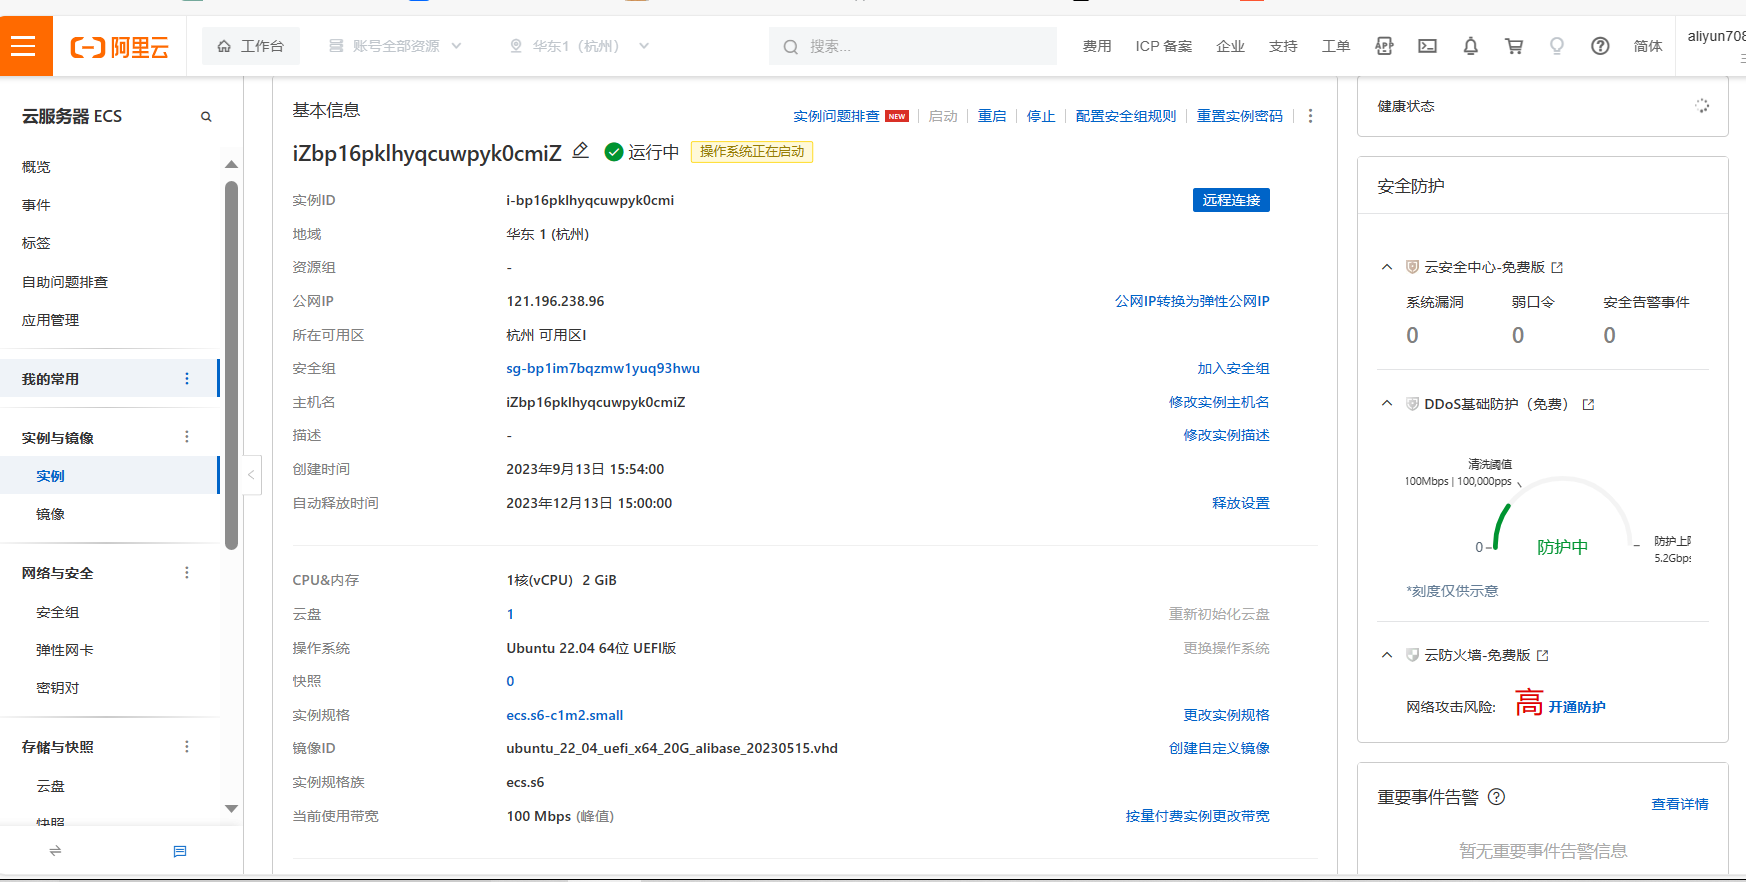
\includegraphics[width=9.5cm,height=8cm]{阿里ESC.png}
\end{figure} 

\clearpage % 强制图片开始新页面

\subsection*{基于 workbench 登录到云实例界面}
\begin{figure}[htbp]
    \centering
    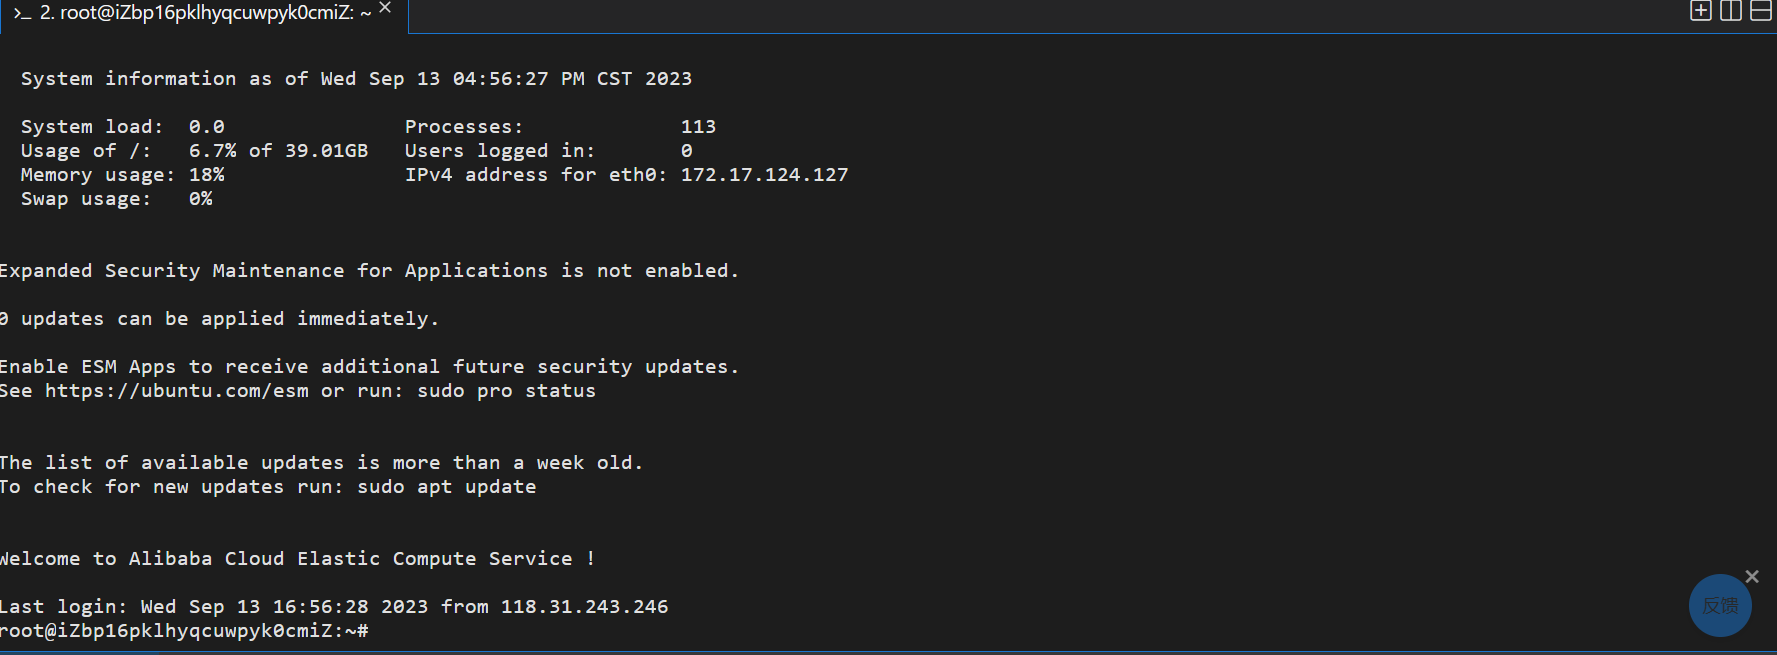
\includegraphics[width=11cm,height=8cm]{登录云实例.png}
\end{figure} 

\subsection*{基础软件下载和环境搭建}
\begin{itemize}
    \item \textbf{Java:} openjdk11.0.20.1
    \item \textbf{系统版本:} Ubuntu20.04
    \item \textbf{Hadoop:} 目标安装版本为 3.3.6 (\verb|wget https://mirrors.aliyun.com/apache/hadoop/core/hadoop-3.3.6/hadoop-3.3.6.tar.gz|)(解压:\verb|tar -xvzf hadoop-3.3.6.tar.gz|)
    \item \textbf{Scala:} 目标安装版本为 2.12.2 
    \item \textbf{Spark:} 目标安装版本为 3.4.1 (适用于 Hadoop 3.3.0 以上版本)(\verb|wget https://mirrors.aliyun.com/apache/spark/spark-3.4.1/spark-3.4.1-bin-hadoop3.tgz|)(解压:\verb|tar -xvzf spark-3.4.1-bin-hadoop3.tgz|)
\end{itemize}

搭建的主要流程:
以下步骤来配置环境:
\begin{enumerate}
    \item \textbf{环境配置:} 参照 \verb|https://blog.csdn.net/weixin_44177980/article/details/130662138|
    \item \textbf{用户配置:} 上面的是新建一个非 root 用户的,如果 root 已经配好了可以参照 \verb|https://blog.csdn.net/white_light/article/details/129411106?spm=1001.2101.3001.6650.2&utm_medium=distribute.pc_relevant.none-task-blog-2%7Edefault%7EBlogCommendFromBaidu%7ERate-2-129411106-blog-8491657.235%5Ev38%5Epc_relevant_sort&depth_1-utm_source=distribute.pc_relevant.none-task-blog-2%7Edefault%7EBlogCommendFromBaidu%7ERate-2-129411106-blog-8491657.235%5Ev38%5Epc_relevant_sort&utm_relevant_index=5| 但是要注意提前给 root 分配 SSH 密码,以后链接都要用上,这个详细参照本条目第一个链接。然后就终于配好了,Hadoop,启动!
\end{enumerate}
\subsection*{配置环境的主要流程:}
\begin{enumerate}
    \item \textbf{配置环境变量:} 编辑 \verb|~/.bashrc| 文件并添加以下内容:
    
    \begin{verbatim}
   export SPARK_HOME=~/spark-hadoop/spark-3.4.1-bin-hadoop3
   export HADOOP_HOME=~/spark-hadoop/hadoop-3.3.6
   export PATH=$SPARK_HOME/bin:$HADOOP_HOME/bin:$PATH
   export PATH=~/spark-hadoop/hadoop-3.3.6/sbin
    \end{verbatim}

   这将设置 Spark 和 Hadoop 的环境变量,使它们可以在终端中使用。使用以下命令将这些配置应用到当前终端:

    \begin{verbatim}
   source ~/.bashrc
    \end{verbatim}
    
    \item \textbf{配置 Hadoop:} 进入 Hadoop 目录,并编辑 `hadoop-env.sh` 文件:
   
    \begin{verbatim}
   cd ~/spark-hadoop/hadoop-3.3.6/etc/hadoop/
   nano hadoop-env.sh
    \end{verbatim}

    在文件中,找到以下行:
   
    \begin{verbatim}
   # export JAVA_HOME=/usr/lib/jvm/java-11-openjdk-amd64
    \end{verbatim}

    取消注释并确保 \texttt{JAVA\_HOME} 的路径正确。保存并退出文件。

    \item \textbf{格式化 Hadoop 文件系统:} 在终端中,使用以下命令格式化 Hadoop 文件系统:

    \begin{verbatim}
   hdfs namenode -format
    \end{verbatim}

   这将准备 HDFS 文件系统以供使用。

    \item \textbf{启动 Hadoop:} 参照前述步骤,先配置那些东西,然后给 root 配置 SSH。使用以下命令启动 Hadoop:

    \begin{verbatim}
   start-dfs.sh
   start-yarn.sh
    \end{verbatim}

   这将启动 Hadoop 的 NameNode、DataNode 和 YARN ResourceManager。

    \item \textbf{验证 Hadoop:} 使用以下命令来验证 Hadoop 是否正常运行:

    \begin{verbatim}
   jps
    \end{verbatim}

    您应该看到输出中包含 NameNode、DataNode、ResourceManager 等进程。

    \item \textbf{启动 Spark:} 使用以下命令启动 Spark:

    \begin{verbatim}
   bash
   ~/spark-hadoop/spark-3.4.1-bin-hadoop3/sbin/start-master.sh
   ~/spark-hadoop/spark-3.4.1-bin-hadoop3/sbin/start-worker.sh
    \end{verbatim}

   这将启动 Spark 的主节点和工作节点。

    \item \textbf{验证 Spark:} 打开浏览器并访问 http://localhost:8080,您应该能够看到 Spark 的 Web UI,显示有关 Spark 集群的信息。
\end{enumerate}

\subsection*{Scala 代码运行结果}
\textbf{这里也有点小坑,Ubuntu 默认没有 Scala 解释器,要先用 scalac 编译 .scala 文件,然后在使用 scala 执行可执行文件。(代码很简单,就不放出来了)}
\begin{figure}[htbp]
    \centering
    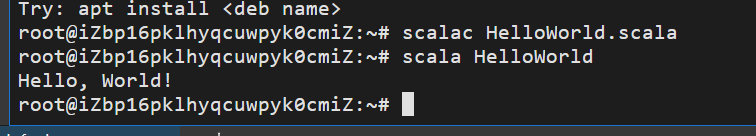
\includegraphics[width=16cm,height=6cm]{firstScala.png}
\end{figure} 

\end{document}
